\chapter{Modellierung \label{Chapter-Methods}}

Um die verschiedenen Modelle testen zu können, werden zwei Ansätze vorgestellt, welche jeweils auf zwei Datensätzen
 trainiert werden. Diese wurden dabei durch ein Simulations-Tool erzeugt, welches im Folgenden erklärt wird.

\section{Datensatz}

\subsection*{WNTR Simulation}

Grundlage für das Trainieren und Evaluieren der Modelle bilden Simulationen des Water Network Tool for Resilience
 (WNTR) \cite{klise2018overview} Auf Basis eines EPANET-Netzwerkes können durch die mannigfaltigen
 Umgebungsvariablen, welche Parameter, wie das zugrunde liegende Hydraulikmodell, aber auch Ereignisse, wie
 Rohrbrüche verschiedenster Stärken, einschließen, eine vielzahl an Szenarien erstellt werden. So besteht der erste
 Datensatz aus ad-hoc generierten, einfachen Szenarien, die durch ihre geringere Komplexität einen schnellen
 Evaluationszyklus gewähren. Hingegen besteht der zweite Datensatz aus vorgenerierten Szenarien, welche mit
 Unsicherheiten und weiter definierten Bedarf, weitaus realistischere Daten darstellen.
 Beide Datensätze nutzen das gleiche WDN als Basis:
 Das sogenannte EPANET Example Network 1 (auch als Net1 zu finden). Dessen Topologie ist in Abbildung
 \ref{fig:practice-wdn} gezeigt und besitzt als verhältnismäßig kleines Netzwerk neun Knotenpunkte, einen Tank
 und ein Reservoir.

\begin{figure}
    \centering
    \fbox{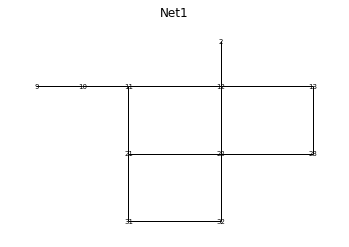
\includegraphics[width=0.7\textwidth]{res/practice-wdn}}
    \caption{Aufbau des Netzwerkes.}
    \label{fig:practice-wdn}
\end{figure}

\subsubsection*{Der ad-hoc Datensatz}

Die Ausgabe der WNTR-Simulation ist eine einfache Tabelle, in welcher für jeden Knoten stündlich die Werte des
 Wasserdrucks eingetragen sind. Abbildung \ref{fig:practice-sim} zeigt einen Beispielverlauf der Druckwerte im Normalzustand sowie
 in Leckszenarien verschiedener Stärken. Diese können mit der Funktion
 \begin{center}
    \texttt{add\_leak(network, area, start\_time, end\_time)},
 \end{center}
 wobei “area” als betroffene Größe in Metern die Stärke
 des Lecks kennzeichnet, zu einem Knoten hinzugefügt werden. Die finalen Einstellungen sehen eine zufällige Stärke
 im Bereich von 0.0009 bis 0.0014 vor. Betrachtet man die Werte der Knoten zu einem bestimmten Zeitpunkt am Tag,
 so sieht man, dass (nach einer bis zu zehntägigen Eingewöhnungsphase, welche im weiteren Verlauf herausgeschnitten
 wird) diese exakt gleich sind. Damit die Modelle nicht die genauen Werte lernen, wird ein geringes,
 normalverteiltes Rauschen hinzu addiert (siehe Abbildung \ref{fig:practice-noise}).

\begin{figure}[h]
    \centering
    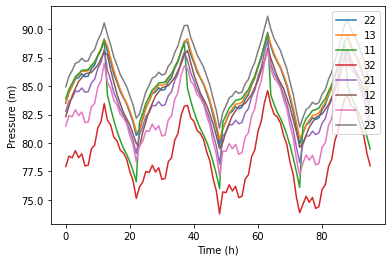
\includegraphics[width=0.45\textwidth]{res/practice-sim-noleak.png}
    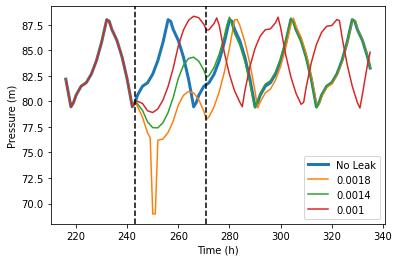
\includegraphics[width=0.45\textwidth]{res/practice-sim-leak.png}
    \caption{Beispielhafte Druckverläufe. Links ein leckfreies Szenario für eine Auswahl an Knoten. Rechts
        für den Knoten 12 ein Vergleich verschiedener Stärken des Lecks.}
    \label{fig:practice-sim}
\end{figure}

\begin{figure}[h]
    \centering
    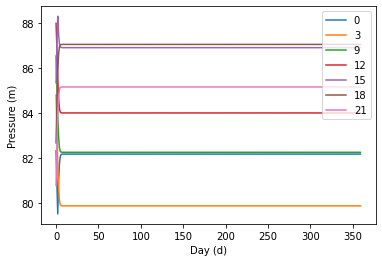
\includegraphics[width=0.44\textwidth]{res/practice-noise-days.png}
    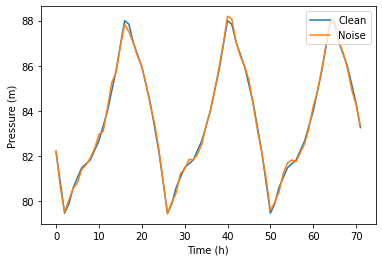
\includegraphics[width=0.44\textwidth]{res/practice-noise-applied.png}
    \caption{Beispielhafte Druckverläufe des Knotens 12. Links sind die Druckwerte ausgewählter Stunden über das
        Jahr angegeben. Nach der Eingewöhnungsphase sind ide vollständig konstant. Rechts ist der Einfluss des
        kleinen Rauschens gezeigt.}
    \label{fig:practice-noise}
\end{figure}

\subsubsection*{LeakDB}

Der realistischere Datensatz LeakDB \cite{vrachimis2018leakdb} ist eine Ansammlung von 1000 Szenarien, welche
 jeweils über ein Jahr andauern und eine doppelt so hohe, zeitliche Auflösung, also halbstündlich, haben.
 Betrachtet man hier ebenso den Verlauf des Wertes einer Tageszeit, so kann man, im Vergleich zum ad-hoc
 Datensatz, hier saisonale Ereignisse und die Unsicherheit direkt erkennen.

\subsection*{Datenformat}

Damit die Daten weiterhin als Zeitfolgen betrachtet werden können, gleichzeitig aber auf mehreren Szenarien
 trainieren und evaluieren werden kann, ist der Definitionsbereich des Modells nicht als $\mathbb{R}^{N \times d}$
 definiert, wobei $N$ die Anzahl an Datenpunkten und $d$ die Anzahl Sensoren ist, sondern als
 $\mathbb{R}^{N \times p \times d}$, mit $p$ als Datenpunkte pro Zeitfolge\footnote{Wichtig anzumerken ist hier,
 dass das $p$ kein fester Wert ist, sondern unterschiedlich für jede der $N$ Zeitfolgen sein kann.} und $N$
 als Anzahl Zeitfolgen. Damit kann dem Modell eine Liste an Zeitfolgen übergeben werden,
 dessen Rückgabewert aus $\{0, 1\}^{N \times p}$ ist, also jedem Zeitpunkt das Label 0 oder 1, für kein Leck
 oder Leck, gibt. Im Folgenden bezeichnet $\mathcal{X}$ diese Liste an Zeitfolgen,
 $X_i \in \mathcal{X}$ eine einzelne Zeitfolge und $x_{i, j} = (x_{i, j}^{(1)}, \dots, x_{i, j}^{(d)}) \in X_i$ den $j$-ten
 Zeitpunkt aus Zeitfolge $i$ mit $x_{i, j}^{(k)}$ als dessen $k$-ten Sensorwert.

Die Analyse für die Metriken, welche aus der
 Konfusionsmatrix berechnet werden, geschieht nun nicht auf den einzelnen Zeitpunkten $x_{i, j}$, sondern auf
 den Zeitfolgen $X_i$. Eine Zeitfolge gilt als Leck-Szenario mit Label 1, falls mindestens ein Zeitpunkt
 innerhalb des Szenarios als Leck gekennzeichnet wurde. Andernfalls bekommt die leckfreie Folge das Label 0.
 Mit diesen Werten kann nun die Konfusionsmatrix gebildet und die Metriken berechnet werden. Ein weiterer Vorteil
 der Betrachtung der Datenpunkte als Liste an Zeitfolgen ist die Berechnung der Detektionszeit: Diese kann nun
 innerhalb einer Zeitfolge als zeitliche Differenz des Auftretens eines Lecks bis hin zu seiner Erkennung gesehen
 werden, gegeben es existiert ein Leck, welches auch wirklich gefunden wurde. Die Menge an Differenzen kann dann
 hinsichtlich Mittelwert, Standardabweichung und Median untersucht werden.

Ein weiterer Schritt beim Vorbereiten der Daten ist das hinzufügen von Zeitinformationen. Während die aus der
 Simulation hervorgehenden Druckwerte nur mit Zeitschritt, also einer natürlichen Nummerierung, indiziert sind,
 ist für die weitere Bearbeitung der Werte eine weitere Informationen benötigt: Die Uhrzeit (im Quellcode auch
 \texttt{hour of the day}) wird durch das Anwenden von \texttt{modulo 24} auf den ursprünglichen
 Index\footnote{Aufgrund der doppelten, zeitlichen Auflösung muss für LeakDB dieser Index noch halbiert werden,
 bevor Modulo gerechnet werden kann.} berechnet und kann damit die Zeitliche Einordnung, welche aus der
 Datenanalyse als annähernd periodisch angesehen ist, erleichtern.


\section{Algorithmen}

Die im Rahmen dieser Arbeit bearbeiteten Strategien sind die der direkten Klassifikation, welche als Baseline
 dienen wird, und der Regressions-Ensemble mit anschließender Threshold-Klassifikation, welche ein weitaus
 solideres Ergebnis liefern soll. Für beide Fälle ist ein Wrapper geschrieben, der neben eigenen Hyperparametern
 ein ML Modell (im Folgenden Basemodel genannt) entgegen nimmt. Dieses ist eines der im Kapitel \ref{Chapter-ML}
 beschriebenen, bekannten Algorithmen. Die Aufgabe des Wrappers ist es, die erhaltenen Daten vor- und
 nachzubereiten, damit sie auf die Basemodels angewendet werden können. Für die Strategie der Klassifikation
 werden sie also so vorbereitet, dass Klassifikationsalgorithmen wie kNN angewendet werden können, während für
 die Strategie des Regressions-Ensemble Algorithmen wie LR oder Ridge angewendet werden.

\subsection*{Klassifikation}

Für die Klassifikation wird ein naiver Ansatz benutzt, in dem ein Klassifikationsmodell auf den rohen Daten
 trainiert und vorhersagt. Dafür werden im Trainingsprozess zuerst die einzelnen Zeitfolgen konkateniert, da
 die Information über die Zeitfolgen hier nicht von Gewicht sind. Die eingabe des Formats
 $\mathbb{R}^{(N*p) \times d}$ wird nun mit den ebenso konkatenierten Labels dem Basemodel zum Trainieren
 bereitgestellt, was den Trainingsprozess beendet. Im Vorhersageprozess wird nun jede eingegebene Zeitfolge
 in das Basemodel eingegeben und die Ergebnisse in eine Ausgabeliste gesteckt. Bevor die Vorhersagen nun
 zurückgegeben werden können, wird ein Median-Filter auf die einzelnen Zeitfolgen angewendet. Dieser geht
 über jeden Wert und setzt in auf den Median der Einträge in einer kleinen Nachbarschaft um den Wert herum.
 So wird beispielsweise ein Zeitpunkt, welcher aufgrund von Rauschen als Leck gelabelt wurde, um sich herum
 jedoch nur leckfreie Zeitpunkte hat, selber zu einem leckfreien Punkt korrigiert. Die größe dieses Zeitfensters
 ist ein Hyperparameter des Wrappers, namentlich \texttt{medfilt\_kernel\_size}.

\subsection*{Regression}

Die Ausgabe der Leckdetektion ist eine binäre Klassifikation. Regressionsalgorithmen können hier dennoch helfen,
 um die Werte des Netzwerks zu einem bestimmten Zeitpunkt zu schätzen und anhand dessen und den real gemessenen
 Werten eine binäre Entscheidung zu fällen. Dieser Prozess ist in Abbildung \ref{fig:practice-ensemble} schematisch
 gezeigt und kann in zwei Phasen eingeteilt werden: Das Generieren des digitalen Zwillings, also die geschätzten
 Druckwerte des gesamten Netzwerkes, mittels Regressions-Ensemble und Klassifikation durch erkannte Thresholds.

\begin{figure}
    \centering
    \fbox{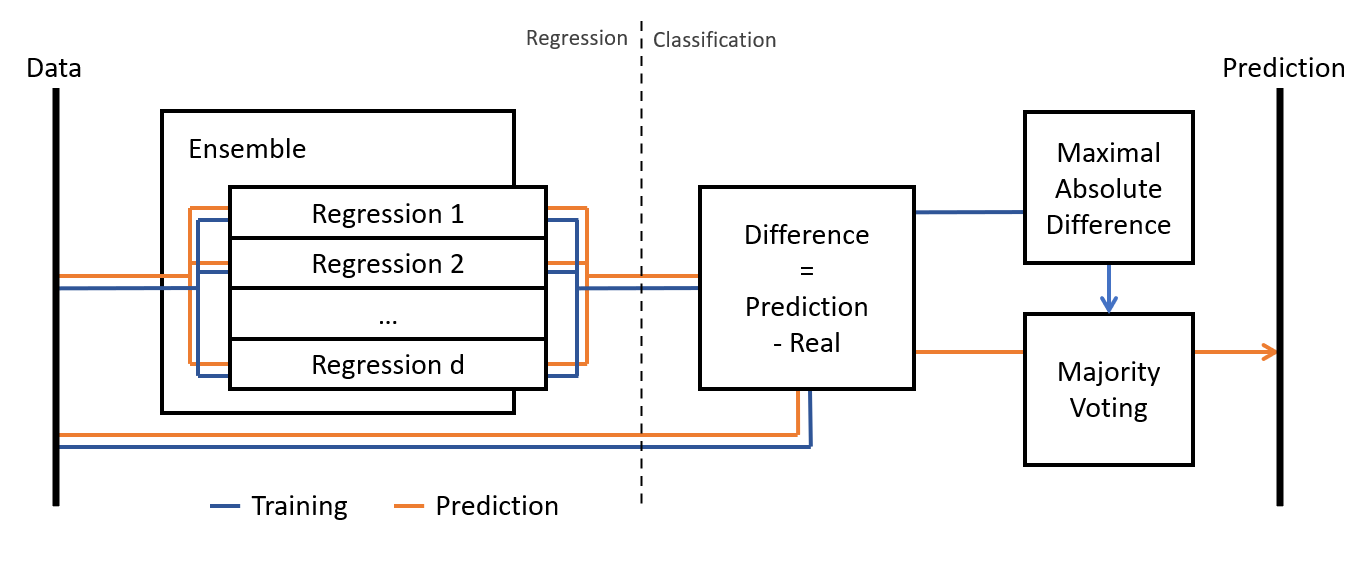
\includegraphics[width=0.9\textwidth]{res/practice-ensemble.png}}
    \caption{Schematische Darstellung des Regression-Ensemble-Ansatzes eingeteilt in die zwei Phasen.}
    \label{fig:practice-ensemble}
\end{figure}

Im Trainingsschritt werden die Listen an Zeitfolgen wie auch beim Klassifikationsansatz zuerst konkateniert.
 Diese Menge an Zeitpunkten wird nun in ein Ensemble an Regressionsalgorithmen geleitet. Dieses ist wie folgt
 aufgebaut:

\begin{itemize}
    \item Für jeden zu schätzenden Knoten gibt es genau einen Regressionsalgorithmus, welcher den Wert des Knoten
     schätzen soll.
    \item Welcher Algorithmus mit welcher Konfiguration der Hyperparameter dies ist, ist als Basemodel festgelegt.
    \item Die Eingabe jedes Basemodels sind die konkatenierten Daten mit jeweiliger Ausnahme der Werte des eigenen
     Knotens\footnote{Wichtig anzumerken ist hier, dass die Daten derart gefiltert werden, dass nur leckfreie
     Zeitpunkte für dieses Training genutzt werden. Im Kapitel \ref{Chapter-Discussion} wird dies weiter
     diskutiert.}.
\end{itemize}

Ist das Ensemble trainiert, wird es direkt benutzt um den digitalen Zwilling zu erschaffen. Die zweite Phase
 beginnt nun damit, die Differenzen zwischen realen und geschätzten Werten zu berechnen. Hierfür werden die
 geschätzten Werte einzeln von ihrem realen Gegenstück abgezogen. Es entsteht eine Differenzenmatrix
 $\mathcal{D} \in \mathbb{R}^{(N*p) \times d}$, die für leckfreie Zeitpunkte vom Betrag niedrige Werte und in
 Szenarien mit Leck hohe Werte haben soll. Um nun Thresholds zu berechnen wird für jeden Knoten die vom Betrag
 her maximale Differenz ausgewählt, welche einem leckfreien Zeitpunkt zugeordnet ist. Mit dem Hyperparameter
 \texttt{th\_multiplier} kann dieser noch um einen gewissen Prozentsatz vergrößert werden. Ein weiterer wichtiger
 Hyperparameter ist der \texttt{th\_mode}, welcher die Werte \texttt{simple} oder \texttt{daytime} annehmen kann.
 Der eben beschriebene Ablauf der Thresholdfindung ist die einfache Berechnung, während die Einstellung
 \texttt{daytime} die Differenzen zusätzlich nach der Tageszeit gruppiert. Während der Threshold-Vektor bei der
 einfachen Berechnung aus $\mathbb{R}^d$ ist, ist dieser nun aus $\mathbb{R}^{d \times tspd}$, wobei $tspd$ die
 Zeitschritte pro Tag angibt, also 24 bei dem ad-hoc Datensatz und 48 bei LeakDB.

Wie bei dem Klassifikationsansatz wird im Vorhersageschritt nun jede Zeitfolge einzeln betrachtet und dessen
 Ergebnisse nach Anwendung des Median-Filters in eine Ausgabeliste eingesetzt. Das Betrachten einer Zeitfolge
 sieht so aus, dass in der ersten Phase wieder mittels Regressions-Ensemble das geschätzte Netzwerk generiert
 und in der folgenden Phase mit den echten Werten zu einer Differenzenmatrix gemacht wird. Die im Trainingsschritt
 gefundenen Thresholds werden nun auf $\mathcal{D}$ angewendet. Dafür wird jeder Wert mit seinem Threshold,
 also nach Knoten und möglicherweise Tageszeit, verglichen. Ist der absolute Wert größer, so gibt der Knoten für
 den Zeitpunkt eine 1 aus, sonst würde er eine 0 ausgeben. Werden die Schätzungen der Knoten nun nach Zeitpunkt
 aufsummiert, erhält jeder Zeitpunkt die Anzahl der Knoten, die Alarm schlagen. Mit dem Hyperparameter
 \texttt{th\_majority} kann man einstellen, wieviel Prozent an Knoten warnen müssen, bevor der Zeitpunkt insgesamt
 als Leck gelabelt wird.

\section{Feature Extraction}

Ein weiteres Werkzeug zum Verbessern von Vorhersagen kann das Feature Extractions sein. Das ist eine Form des
 Preprocessings, bei dem die Daten transformiert werden um Features zu entfernen, modifizieren oder hinzuzufügen.
 Zwei in dieser Arbeit untersuchte Methoden werden im Folgenden vorgestellt.

\subsection*{Past Days Transform}

Die Past Days Transform versucht sich die annähernde Periodizität der Daten zu nutze zu machen, die bei
der Analyse der Daten herausgekommen ist. Dafür werden zu den Druckwerten an einem Zeitpunkt die jeweiligen
Druckwerte des letzten Tages hinzugefügt. Ein Datenpunkt sieht dann so aus:

\begin{equation*}
    x_{i, j} = (x_{i, j}^{(1)}, \dots, x_{i, j}^{(d)}, x_{i, j-tspd}^{(1)}, \dots, x_{i, j-tspd}^{(d)})
\end{equation*}

Dies kann rekursiv mehrere Male gemacht werden, wodurch ein Datenpunkt mehrere Tage in die Vergangenheit
 gucken kann. Der Parameter \texttt{past\_end} kontrolliert, wie viele Tage Rückblick betrachtet werden. Ist
 dieser beispielsweise auf Drei, so besitzt ein Datenpunkt die Druckwerte des eigenen Tages, des Tages
 zuvor und die des zwei Tage zurückliegenden Datums.

\subsection*{Mean Transform}

Um Rauschen entgegenzuwirken kann dass Mitteln der Werte in einem kleinen Fenster um die jeweiligen Werte helfen.
 Mean Transform implementiert genau diese Methoden. Dabei kann mit dem Parameter \texttt{window} die Größe des
 Fensters eingestellt werden.
